\documentclass[12pt]{beamer}
\setbeamertemplate{navigation symbols}{}
%\usepackage[latin1]{inputenc}
\usepackage{pgfplots}
\usepackage{adjustbox}
\usepackage{graphicx}
%\usepackage{draftwatermark}
\usepackage{tikz}
\usepackage{subfigure}
\usetheme{Amsterdam}
\usecolortheme{default}
\title[]{The effects of transitions of power on the contents of
	municipal government websites}
\author{Markus Neumann \\ Bruce Desmarais \\ Hanna Wallach \\ Fridolin Linder}
\institute{The Pennsylvania State University}
\date{January 6, 2018}

\makeatletter
\defbeamertemplate*{footline}{myminiframes theme}
{%
	\begin{beamercolorbox}[colsep=1.5pt]{upper separation line foot}
	\end{beamercolorbox}
	\hbox{%
		\begin{beamercolorbox}[wd=.1\paperwidth,ht=2.5ex,dp=1.125ex,%
			leftskip=.3cm,rightskip=.3cm,center]{title in head/foot}%
			{\usebeamerfont{author in head/foot}\usebeamercolor[fg]{author in head/foot}\insertframenumber/\inserttotalframenumber}%
		\end{beamercolorbox}%
		\begin{beamercolorbox}[wd=.75\paperwidth,ht=2.5ex,dp=1.125ex,%
			leftskip=.3cm,rightskip=.3cm plus1fil,center]{title in head/foot}%
			\leavevmode{\usebeamerfont{title in head/foot}\insertshorttitle}%
		\end{beamercolorbox}%
		\begin{beamercolorbox}[wd=.15\paperwidth,ht=2.5ex,dp=1.125ex,%
			leftskip=.3cm,rightskip=.3cm plus1fil,center]{title in head/foot}%
			{\usebeamerfont{author in head/foot}\usebeamercolor[fg]{author in head/foot}\insertshortauthor}
		\end{beamercolorbox}%
	}%
	\begin{beamercolorbox}[colsep=1.5pt]{lower separation line foot}
	\end{beamercolorbox}
}
\makeatother

\begin{document}

\section{Introduction}
\begin{frame}
\titlepage
\end{frame}

%\begin{frame}{Spot the difference}
%\begin{figure}
%	\hfill
%	\subfigure{\includegraphics[width=5cm]{Images/Clinton_Rally_cr.jpg}}
%	\hfill
%	\subfigure{\includegraphics[width=5cm]{Images/Trump_Rally_cr.jpg}}
%\end{figure}
%\end{frame}

\begin{frame}{Government Websites}
\linespread{1.5}
{\large
	\begin{itemize}
	\item Transparency
	\end{itemize}
	}
\end{frame}

\section{Data Collection}
\begin{frame}{wget}
\end{frame}

\section{Preprocessing}

\begin{frame}{Document filetype \& conversion}
\begin{itemize}
	\item Websites contain a number of different filetypes
	\item txt, pdf, html, doc and docx are useable
	\item convert everything to txt
	\item the file ENDING does not always 
\end{itemize}
\end{frame}

\begin{frame}{Duplicate Line Removal}
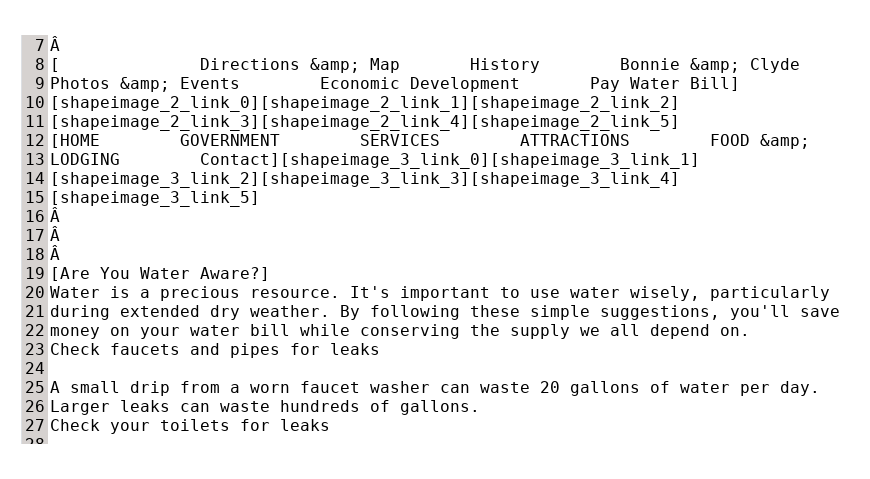
\includegraphics[width = \linewidth]{duplicateLines.png}
\end{frame}

\begin{frame}{Duplicate Line Removal}
	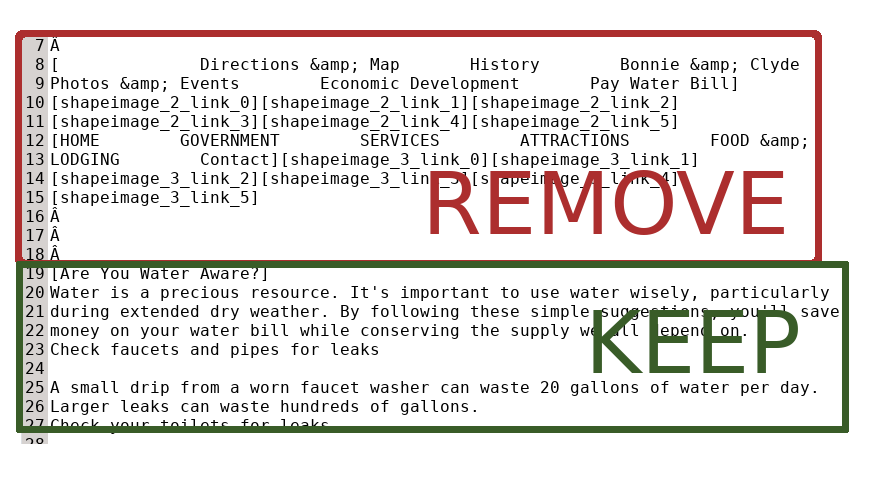
\includegraphics[width = \linewidth]{duplicateLineRemoval.png}
\end{frame}

\begin{frame}{Duplicate Line Removal}
\begin{itemize}
	\item Within each city, there is a lot of shared text
	\begin{itemize}
		\item Boilerplate
		\item Website elements
	\end{itemize}
	\item If not removed, the text clusters into cities
\end{itemize}
\begin{itemize}
	\item Solution: Compare each line in each document to every other line in every document of that city
	\item Count duplicates
	\item Remove a line if it is duplicated within a city above some threshold
	\item Hash tables for computational efficiency
\end{itemize}
\end{frame}

\begin{frame}{Other preprocessing}
\begin{itemize}
	\item Remove:
	\begin{itemize}
		\item Dates
		\item Numbers
		\item Punctuation
		\item Words not recognized by an English dictionary
		\item Stopwords
		\item Documents with too few unique words
	\end{itemize}
\item Set to lowercase
\item Lemmatization
\end{itemize}
\end{frame}

\section{Analysis}
\begin{frame}{Hierarchical Clustering}
\end{frame}

\begin{frame}{Fightin' Words}
\begin{figure}
	\hfill
	\subfigure{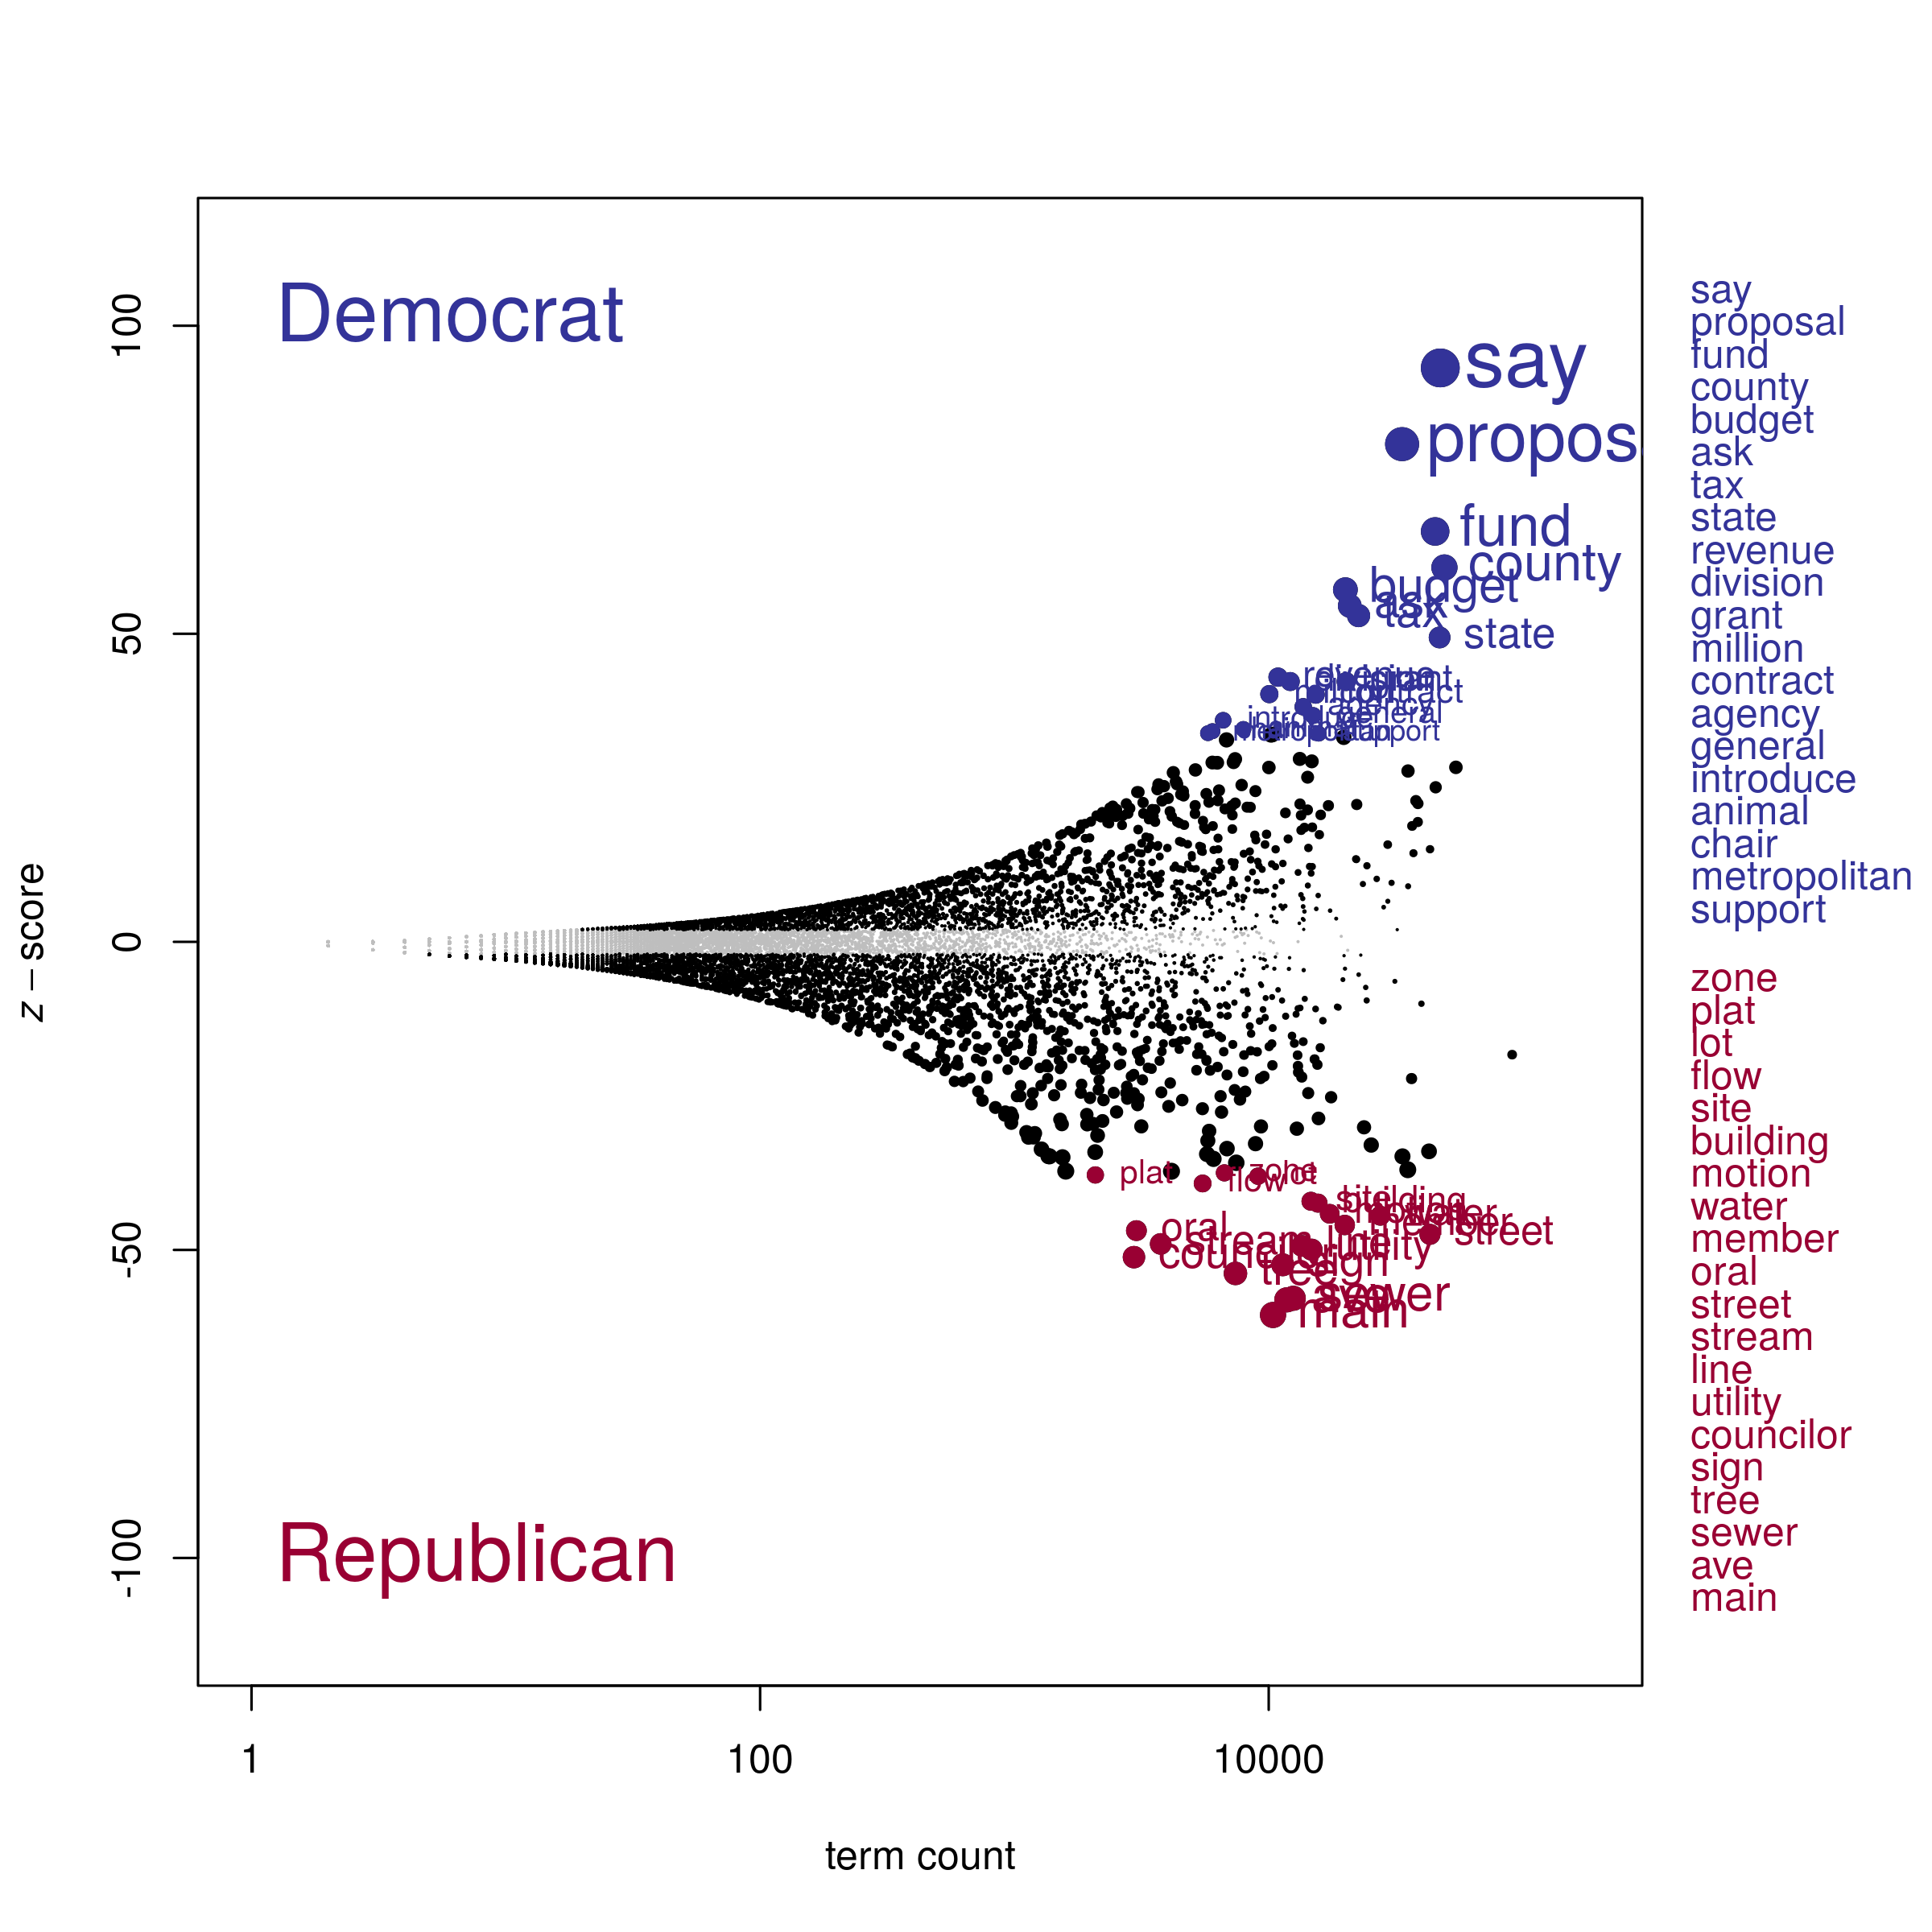
\includegraphics[width=5cm]{../figures/fightinWordsIN.png}}
	\hfill
	\subfigure{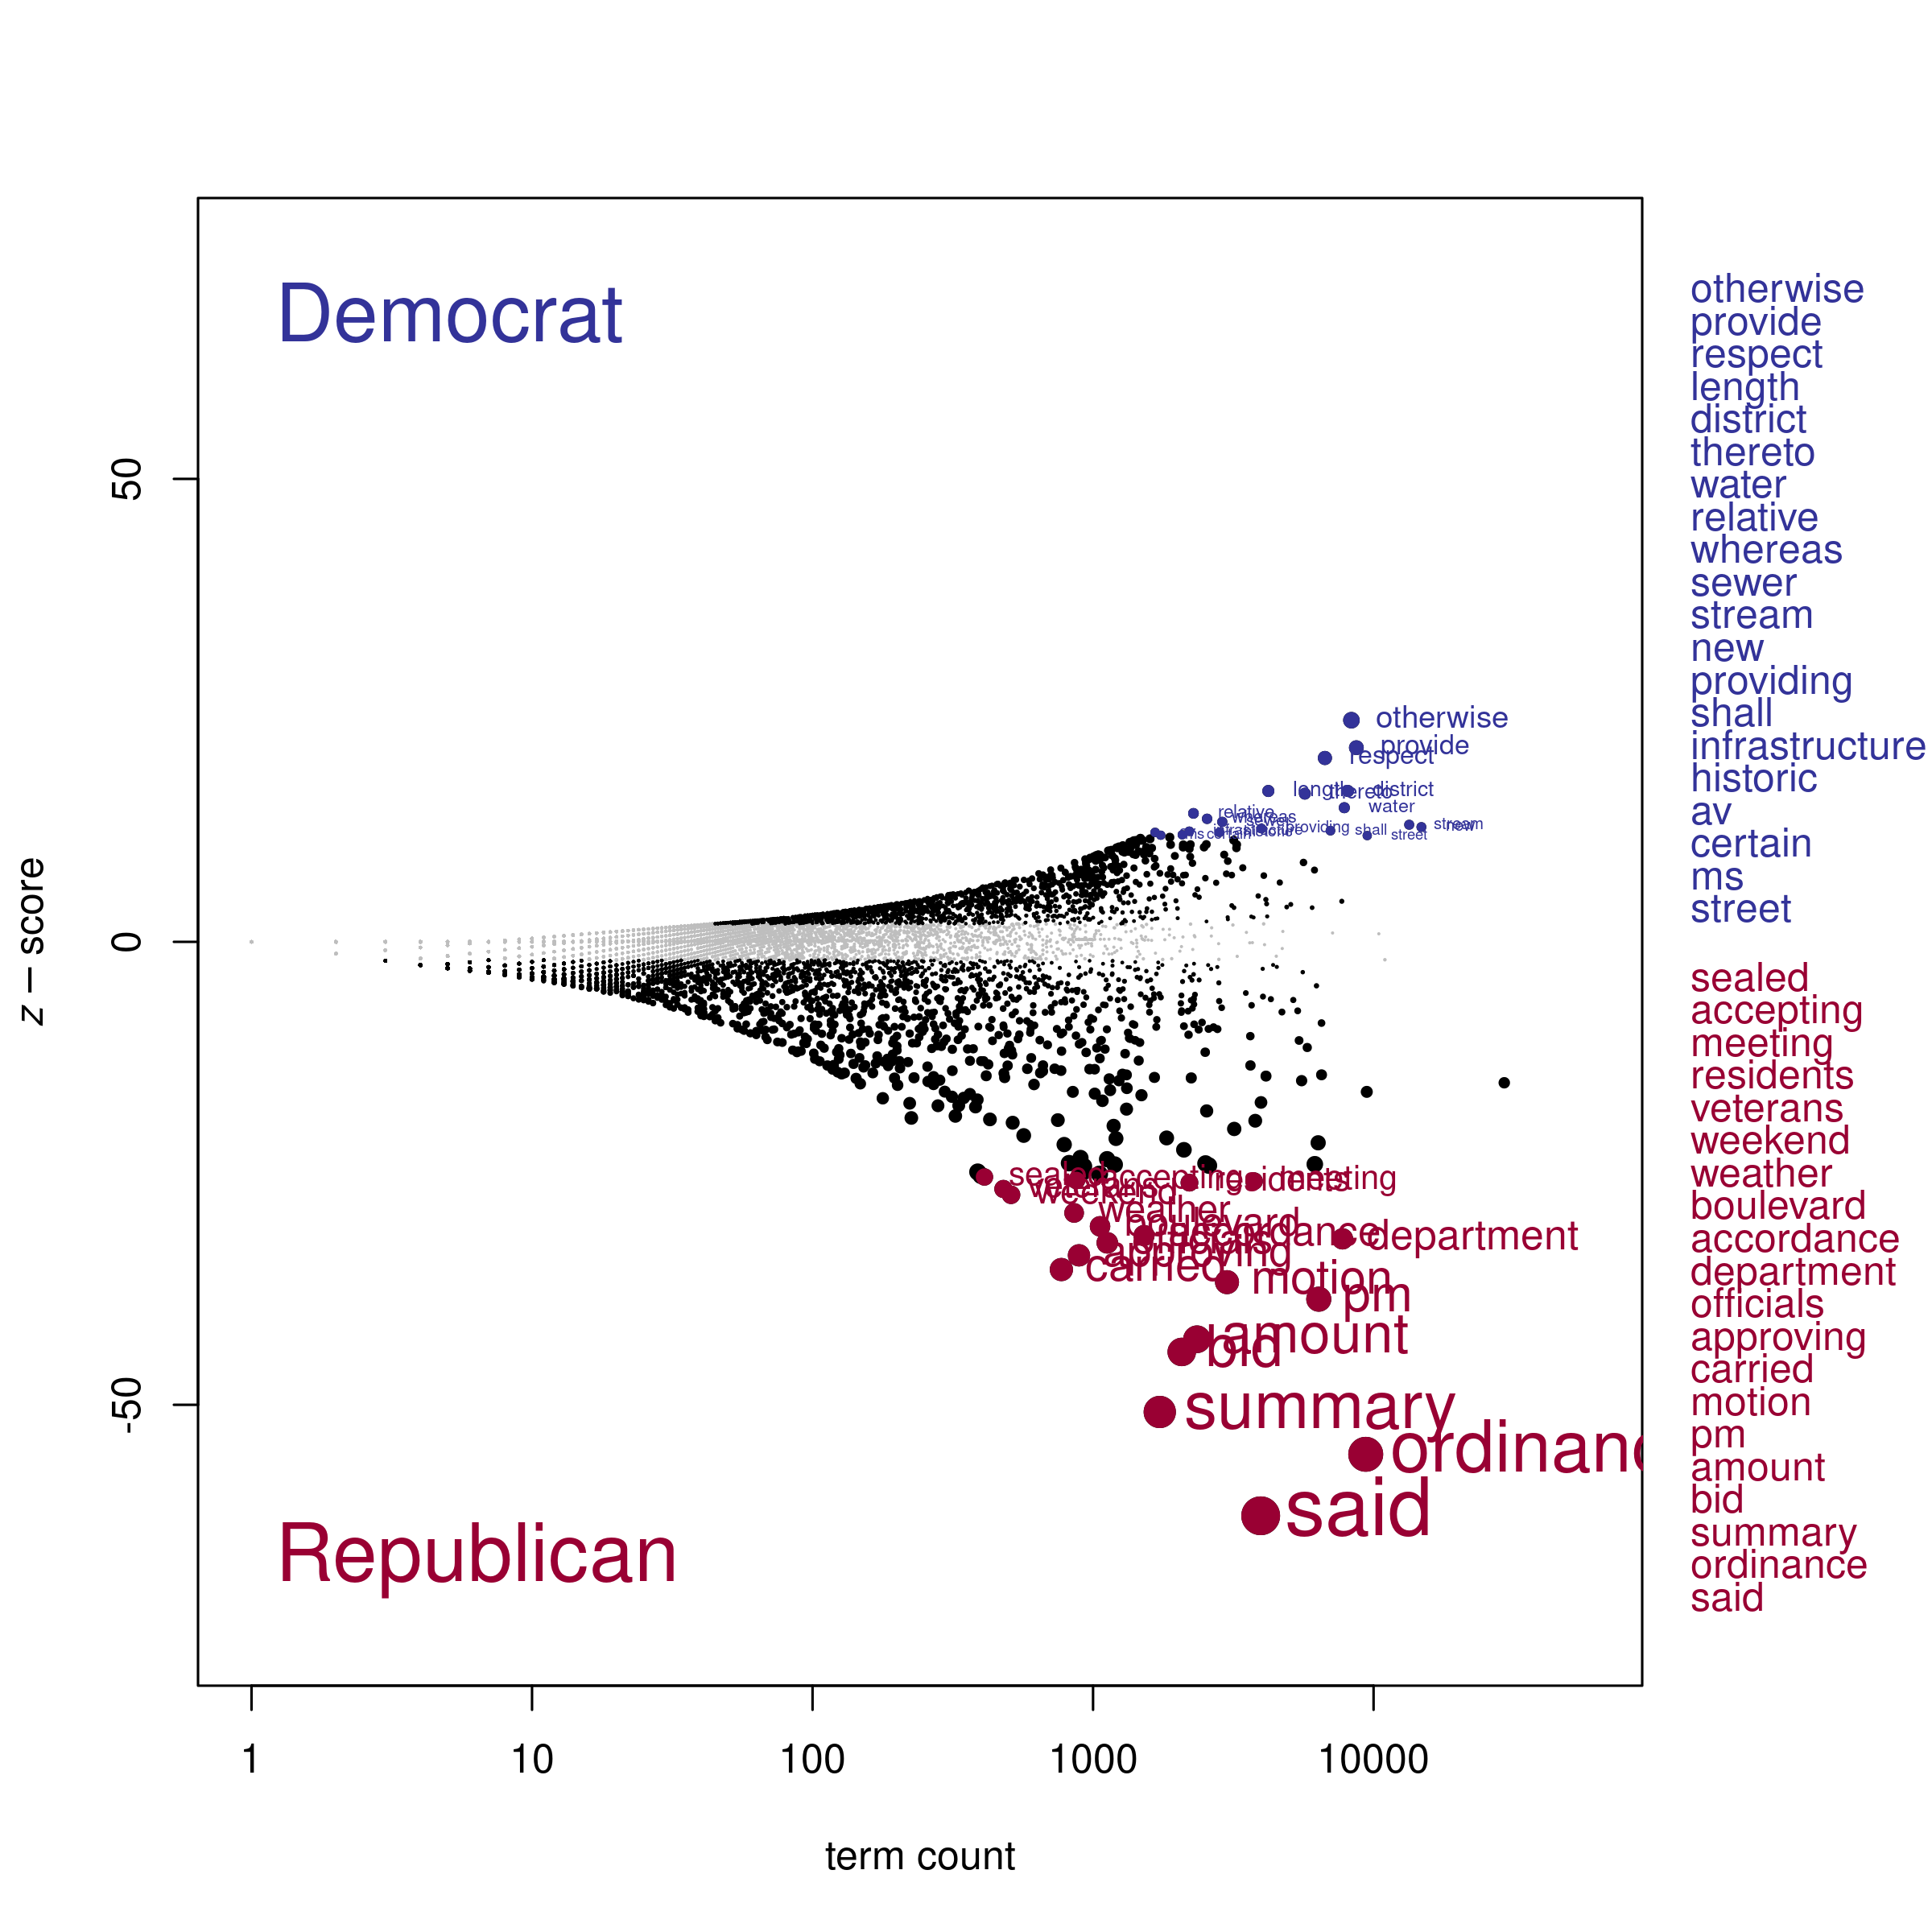
\includegraphics[width=5cm]{../figures/fightinWordsLA.png}}
\end{figure}
\end{frame}

\begin{frame}{Latent Dirichlet Allocation}
\end{frame}

\section{Conclusion}
\begin{frame}{Conclusion}
\end{frame}

\end{document}